\begin{frame}
	\frametitle{2-Qubit Quantum Circuit}
	\only<2>{\framesubtitle{Initialization}}
	\begin{tikzpicture}	
	\node[anchor=south west,inner sep=0] (image) at (0,0) {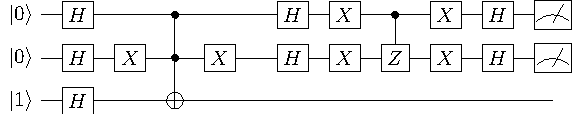
\includegraphics[width=0.9\textwidth]{figures/circuits/2-qubit.pdf}};
	\begin{scope}[x={(image.south east)},y={(image.north west)}]
		%\draw[help lines,xstep=.1,ystep=.1] (0,0) grid (1,1);
		%\foreach \x in {0,1,...,9} { \node [anchor=north] at (\x/10,0) {0.\x}; }
		%\foreach \y in {0,1,...,9} { \node [anchor=east] at (0,\y/10) {0.\y}; }
		\draw<2->[thick,dashed] (0.085,-0.05) rectangle (0.185,1.05);
		\node<2-> [above] at (0.125,1.1) {Initialization};
	\end{scope}

	\end{tikzpicture}	
\end{frame}

\begin{frame}
	\frametitle{2-Qubit Quantum Circuit}
	\framesubtitle{Initialization}
	\begin{eqnarray*}
		\psi^{[0]} & = & \ket{001}\\
		\psi^{[1]} & = & H^{\otimes 3} \psi^{[0]}\\
				   & = & \frac{1}{\sqrt{8}}\left(\ket{000} + \ket{010} + \ket{100} + \ket{110} - \left.\ket{001} - \ket{011} - \ket{101} - \ket{111} \right) \right.\\ 
	\end{eqnarray*}
\end{frame}

\begin{frame}
	\frametitle{2-Qubit Quantum Circuit}
	\framesubtitle{Quantum Oracle}
	\begin{tikzpicture}	
	\node[anchor=south west,inner sep=0] (image) at (0,0) {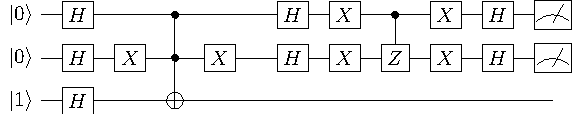
\includegraphics[width=0.9\textwidth]{figures/circuits/2-qubit.pdf}};
	\begin{scope}[x={(image.south east)},y={(image.north west)}]
	%\draw[help lines,xstep=.1,ystep=.1] (0,0) grid (1,1);
	%\foreach \x in {0,1,...,9} { \node [anchor=north] at (\x/10,0) {0.\x}; }
	%\foreach \y in {0,1,...,9} { \node [anchor=east] at (0,\y/10) {0.\y}; }
	\draw<1->[thick,dashed] (0.085,-0.05) rectangle (0.185,1.05);
	\node<1-> [above] at (0.125,1.1) {Initialization};
	
	\draw<1->[thick,dashed] (0.185,-0.05) rectangle (0.45,1.05);
	\node<1-> [above] at (0.3125,1.1) {Quantum Oracle};
	\end{scope}
	
	\end{tikzpicture}	
\end{frame}

\begin{frame}
	\frametitle{2-Qubit Quantum Circuit}
	\framesubtitle{Quantum Oracle}
	
	\begin{eqnarray*}
		U_f & = & \left(I\otimes X \otimes I\right) \cdot T \cdot \left(I\otimes X \otimes I\right) = 
			\begin{pmatrix*}[r]
					1 & 0 & 0 & 0 & 0 & 0 & 0 & 0 \\
					0 & 1 & 0 & 0 & 0 & 0 & 0 & 0 \\
					0 & 0 & 1 & 0 & 0 & 0 & 0 & 0 \\
					0 & 0 & 0 & 1 & 0 & 0 & 0 & 0 \\
					0 & 0 & 0 & 0 & 0 & 1 & 0 & 0 \\
					0 & 0 & 0 & 0 & 1 & 0 & 0 & 0 \\
					0 & 0 & 0 & 0 & 0 & 0 & 1 & 0 \\
					0 & 0 & 0 & 0 & 0 & 0 & 0 & 1
		    \end{pmatrix*}
	\end{eqnarray*}
\end{frame}

\begin{frame}
	\frametitle{2-Qubit Quantum Circuit}
	\framesubtitle{Quantum Oracle}
	
	\begin{eqnarray*}
		\psi^{[1]} & = &\frac{1}{\sqrt{8}}\left(\ket{000} + \ket{010} + \ket{100} + \ket{110} - \ket{001} - \ket{011} - \ket{101} - \ket{111} \right) \\  
		\psi^{[2]} & = & U_f\ket{\psi^{[1]}}\\
				   & = & \frac{1}{\sqrt{8}}\left(\ket{000} + \ket{010} + \ket{101} + \ket{110} - \ket{001} - \ket{011} - \ket{100} - \ket{111} \right) \\  
				   & = & \frac{1}{\sqrt{8}}\left(\ket{00} + \ket{01} - \ket{10} + \ket{11}\right)\otimes\left(\ket{0} - \ket{1}\right) \\
				   & = & \frac{1}{2}\left(\ket{00} + \ket{01} - \ket{10} + \ket{11}\right)\otimes\frac{1}{\sqrt{2}}\left(\ket{0} - \ket{1}\right)
	\end{eqnarray*}
\end{frame}

\begin{frame}
	\frametitle{2-Qubit Quantum Circuit}
	\framesubtitle{Difussion Operator}
	\begin{tikzpicture}	
	\node[anchor=south west,inner sep=0] (image) at (0,0) {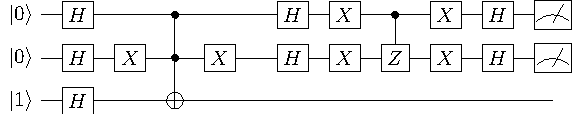
\includegraphics[width=0.9\textwidth]{figures/circuits/2-qubit.pdf}};
	\begin{scope}[x={(image.south east)},y={(image.north west)}]
	%\draw[help lines,xstep=.1,ystep=.1] (0,0) grid (1,1);
	%\foreach \x in {0,1,...,9} { \node [anchor=north] at (\x/10,0) {0.\x}; }
	%\foreach \y in {0,1,...,9} { \node [anchor=east] at (0,\y/10) {0.\y}; }
	\draw<1->[thick,dashed] (0.085,-0.05) rectangle (0.185,1.05);
	\node<1-> [above] at (0.125,1.1) {Initialization};
	
	\draw<1->[thick,dashed] (0.185,-0.05) rectangle (0.45,1.05);
	\node<1-> [above] at (0.3125,1.1) {Quantum Oracle};
	
	\draw<1->[thick,dashed] (0.45,-0.05) rectangle (0.912,1.05);
	\node<1-> [above] at (0.7,1.1) {Difussion operator};
	\end{scope}
	
	\end{tikzpicture}	
\end{frame}

\begin{frame}
	\frametitle{2-Qubit Quantum Circuit}
	\framesubtitle{Diffusion Operator}
	
	\begin{eqnarray*}
		U_d & = & \left(H\otimes H\right) \cdot \left(X\otimes X\right)\cdot \left(CZ\right) \left(X\otimes X\right) \cdot \left(H \otimes H \right) =  \frac{1}{4}
		\begin{pmatrix*}[r]
			2 & -2 & -2 & -2 \\
			-2 & 2 & -2 & -2 \\
			-2 & -2 & 2 & -2 \\
			-2 & -2 & -2 & 2
		\end{pmatrix*}
	\end{eqnarray*}
	\begin{eqnarray}
		&& \psi^{[3]} = U_d\psi^{[2]}\nonumber\\
		           &&\frac{1}{8}
		           \begin{pmatrix*}[r]
		           2 & -2 & -2 & -2 \\
		           -2 & 2 & -2 & -2 \\
		           -2 & -2 & 2 & -2 \\
		           -2 & -2 & -2 & 2
		           \end{pmatrix*}
		           \begin{pmatrix*}[r]
		           1 & 0 & 0 & 0 \\
		           0 & 1 & 0 & 0 \\
		           0 & 0 & -1 & 0 \\
		           0 & 0 & 0 & 0
		           \end{pmatrix*}=\frac{1}{8}
		           \begin{pmatrix*}[r]
		           2 & -2 & 2 & -2 \\
		           -2 & 2 & 2 & -2 \\
		           -2& -2 & -2 & -2 \\
		           -2 & -2 & 2 & 2
		           \end{pmatrix*}\rightarrow
		           \begin{pmatrix*}[r]
		           0\\
		           0 \\
		           -1\\
		           0
		           \end{pmatrix*} = -\ket{10}\nonumber
	\end{eqnarray}
		
\end{frame}
			